\documentclass[11pt,a4paper]{article}
\usepackage[margin=2.4cm]{geometry}
\usepackage{amsmath,amssymb}
\usepackage{algorithm}
\usepackage{algpseudocode}
\usepackage{booktabs}
\usepackage{etoolbox}
\usepackage{pgfplots}
\pgfplotsset{compat=1.17}
\usepackage[hidelinks]{hyperref}
\usepackage{cleveref}

\AtBeginEnvironment{algorithmic}{\small}
\newcommand{\id}[1]{\texttt{#1}}
\newcommand{\nnz}{\mathrm{nnz}}

\title{Matrix--Vector Multiplication $y = Ax$:\\ Dense versus CSR Storage}
\author{Gustavo Lozano}
\date{\today}

\begin{document}
\maketitle

\begin{abstract}
The product $y = Ax$ is the core operation of iterative solvers and of most
first-order optimization methods. This document compares two ways of
computing it: with $A$ stored as a dense array and with $A$ stored in
compressed sparse row (CSR) format. For each, we give the algorithm, count
floating-point operations and memory traffic, derive the arithmetic intensity,
estimate run time with the roofline model, find the density at which both
formats cost the same, and discuss parallelization with OpenMP. The main
conclusion is that both computations are limited by memory bandwidth, so the
format that moves fewer bytes wins; for sparse matrices this is CSR by several
orders of magnitude.
\end{abstract}

\tableofcontents

%======================================================================
\section{Problem and notation}
%======================================================================

Given $A \in \mathbb{R}^{M \times N}$ and $x \in \mathbb{R}^{N}$, compute
\[
  y_i = \sum_{j=0}^{N-1} a_{ij}\, x_j, \qquad i = 0, \dots, M-1 .
\]

\begin{center}
\begin{tabular}{ll}
\toprule
Symbol & Meaning \\
\midrule
$M, N$ & number of rows and columns of $A$ \\
$\nnz$ & number of stored nonzero entries of $A$ \\
$n_i$ & number of nonzeros in row $i$, so $\sum_i n_i = \nnz$ \\
$d = \nnz / (MN)$ & density of $A$ \\
$s_v, s_i$ & bytes per value and per index (here $s_v = 8$, double; $s_i = 4$, 32-bit int) \\
$\beta$ & memory bandwidth (bytes/s) \\
$\pi$ & peak floating-point rate (flop/s) \\
\bottomrule
\end{tabular}
\end{center}

\noindent All indices are 0-based. Costs are given for double-precision values
and 32-bit indices.

%======================================================================
\section{Storage formats}
%======================================================================

\subsection{Dense}

All $MN$ entries are stored, zeros included, in one contiguous array.
In \emph{row-major} order (the C convention), $a_{ij}$ is at position
$iN + j$; in \emph{column-major} order (the Fortran and BLAS convention),
it is at position $i + jM$.
\[
  \text{memory}_{\text{dense}} = s_v\, M N \ \text{bytes}.
\]

\subsection{Compressed sparse row (CSR)}

Only the nonzeros are stored, row by row, in three arrays:
\begin{itemize}
  \item $\id{val}[0..\nnz-1]$: the nonzero values;
  \item $\id{col}[0..\nnz-1]$: the column index of each value;
  \item $\id{row\_ptr}[0..M]$: row $i$ occupies positions
        $\id{row\_ptr}[i], \dots, \id{row\_ptr}[i+1]-1$, and
        $\id{row\_ptr}[M] = \nnz$.
\end{itemize}
\[
  \text{memory}_{\text{CSR}} = (s_v + s_i)\,\nnz + s_i (M+1)
  = 12\,\nnz + 4(M+1) \ \text{bytes}.
\]

\subsection{Running example}

\[
A = \begin{pmatrix}
10 & 0 & 0 & 0 & 2 & 0 \\
0  & 3 & 0 & 0 & 0 & 0 \\
0  & 0 & 0 & 0 & 0 & 0 \\
0  & 0 & 7 & 0 & 0 & 1 \\
4  & 0 & 0 & 0 & 0 & 0 \\
0  & 0 & 0 & 5 & 0 & 6
\end{pmatrix},
\qquad
x = \begin{pmatrix} 1 \\ 2 \\ 3 \\ 4 \\ 5 \\ 6 \end{pmatrix},
\qquad M = N = 6,\ \nnz = 8,\ d = \tfrac{8}{36} \approx 0.22 .
\]
The exact product is
\[
y = Ax =
\begin{pmatrix}
10 \cdot 1 + 2 \cdot 5 \\
3 \cdot 2 \\
0 \\
7 \cdot 3 + 1 \cdot 6 \\
4 \cdot 1 \\
5 \cdot 4 + 6 \cdot 6
\end{pmatrix}
=
\begin{pmatrix} 20 \\ 6 \\ 0 \\ 27 \\ 4 \\ 56 \end{pmatrix},
\]
which serves as the reference result for testing any implementation.
Row 2 is empty, which shows how CSR handles rows with no nonzeros.
\begin{align*}
\id{val}     &= [10, 2, 3, 7, 1, 4, 5, 6], \\
\id{col}     &= [0, 4, 1, 2, 5, 0, 3, 5], \\
\id{row\_ptr} &= [0, 2, 3, 3, 5, 6, 8].
\end{align*}

\noindent Storage:
\begin{center}
\begin{tabular}{lrr}
\toprule
Array & Elements & Bytes \\
\midrule
Dense $A$ ($8MN$) & $36$ doubles & 288 \\
\midrule
CSR \id{val} ($8\,\nnz$) & 8 doubles & 64 \\
CSR \id{col} ($4\,\nnz$) & 8 ints & 32 \\
CSR \id{row\_ptr} ($4(M+1)$) & 7 ints & 28 \\
CSR total & & 124 \\
\bottomrule
\end{tabular}
\end{center}

\noindent CSR uses 124 bytes instead of 288, a factor of $2.3$ less, even for
this tiny matrix. Note that the $4(M+1)$ bytes of \id{row\_ptr} do not depend
on $\nnz$: for very small matrices this fixed overhead is noticeable, and a
small matrix needs a density somewhat below the asymptotic break-even
$d^* \approx 2/3$ (\cref{sec:breakeven}) before CSR is smaller.

\subsection{Storage comparison for larger matrices}
\label{sec:storage-comparison}

For a square matrix ($M = N$) the two formulas are
\[
  \text{memory}_{\text{dense}} = 8N^2,
  \qquad
  \text{memory}_{\text{CSR}} = 12\,\nnz + 4(N+1),
\]
and the ratio is
\[
  \rho = \frac{\text{memory}_{\text{dense}}}{\text{memory}_{\text{CSR}}}
       = \frac{8N^2}{12\,\nnz + 4(N+1)} .
\]
Dense storage grows with $N^2$ no matter how many entries are zero; CSR grows
with $\nnz$. Two cases are worth separating.

\paragraph{Fixed number of nonzeros per row.}
Many sparse matrices have about $k$ nonzeros per row whatever their size
(for example $k \approx 5$ for a 2-D finite-difference grid, or a few
variables per constraint in a large optimization model). Then
$\nnz = kN$, CSR grows only linearly, and
\[
  \rho \approx \frac{8N}{12k + 4},
\]
so the saving \emph{grows with the size of the matrix}. For $k = 5$,
$\rho \approx N/8$:

\begin{center}
\begin{tabular}{rrrrr}
\toprule
$N$ & $\nnz = 5N$ & dense & CSR & ratio $\rho$ \\
\midrule
$10^2$ & $5 \cdot 10^2$ & 80 KB & 6.4 KB & 12.5 \\
$10^3$ & $5 \cdot 10^3$ & 8 MB & 64 KB & 125 \\
$10^4$ & $5 \cdot 10^4$ & 800 MB & 640 KB & 1\,250 \\
$10^5$ & $5 \cdot 10^5$ & 80 GB & 6.4 MB & 12\,500 \\
$10^6$ & $5 \cdot 10^6$ & 8 TB & 64 MB & 125\,000 \\
\bottomrule
\end{tabular}
\end{center}

\noindent Beyond
$N \approx 4.5 \cdot 10^4$ the dense matrix no longer fits in 16 GB of memory,
while the CSR matrix still takes only megabytes.

\paragraph{Fixed size, varying density.}
For $N = 10^4$ the dense matrix always takes 800 MB, and CSR depends only on
$\nnz = d N^2$:

\begin{center}
\begin{tabular}{rrrrr}
\toprule
density $d$ & $\nnz$ & dense & CSR & ratio $\rho$ \\
\midrule
$10^{-4}$ & $10^4$ & 800 MB & 0.16 MB & 5\,000 \\
$10^{-3}$ & $10^5$ & 800 MB & 1.24 MB & 645 \\
$10^{-2}$ & $10^6$ & 800 MB & 12.0 MB & 66 \\
$10^{-1}$ & $10^7$ & 800 MB & 120 MB & 6.7 \\
$0.5$     & $5 \cdot 10^7$ & 800 MB & 600 MB & 1.33 \\
$2/3$     & $6.7 \cdot 10^7$ & 800 MB & 800 MB & 1.00 \\
$1$       & $10^8$ & 800 MB & 1\,200 MB & 0.67 \\
\bottomrule
\end{tabular}
\end{center}

\noindent The storage break-even is at $d \approx 2/3$: above it, the 4-byte
index stored with every value makes CSR \emph{larger} than dense.

\begin{figure}[H]
\centering
\begin{minipage}[t]{0.49\textwidth}
\centering
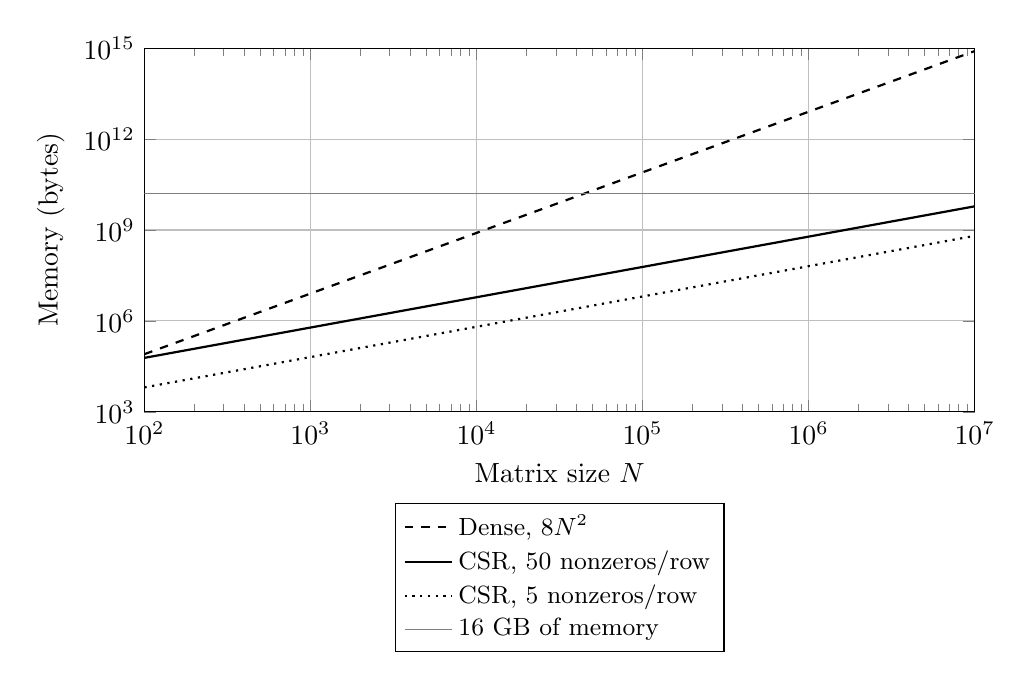
\begin{tikzpicture}
\begin{loglogaxis}[
  width=\textwidth, height=6.2cm,
  xmin=1e2, xmax=1e7, ymin=1e3, ymax=1e15,
  xlabel={Matrix size $N$},
  ylabel={Memory (bytes)},
  ytickten={3,6,9,12,15},
  grid=major, legend cell align=left,
  legend style={at={(0.5,-0.25)}, anchor=north, font=\small}]
\addplot[thick, dashed, domain=1e2:1e7, samples=2] {8*x^2};
\addlegendentry{Dense, $8N^2$}
\addplot[thick, domain=1e2:1e7, samples=2] {604*x+4};
\addlegendentry{CSR, 50 nonzeros/row}
\addplot[thick, dotted, domain=1e2:1e7, samples=2] {64*x+4};
\addlegendentry{CSR, 5 nonzeros/row}
\addplot[thin, gray, domain=1e2:1e7, samples=2] {1.6e10};
\addlegendentry{16 GB of memory}
\end{loglogaxis}
\end{tikzpicture}

\small (a) Memory against size, with $\nnz = kN$.
\end{minipage}\hfill
\begin{minipage}[t]{0.49\textwidth}
\centering
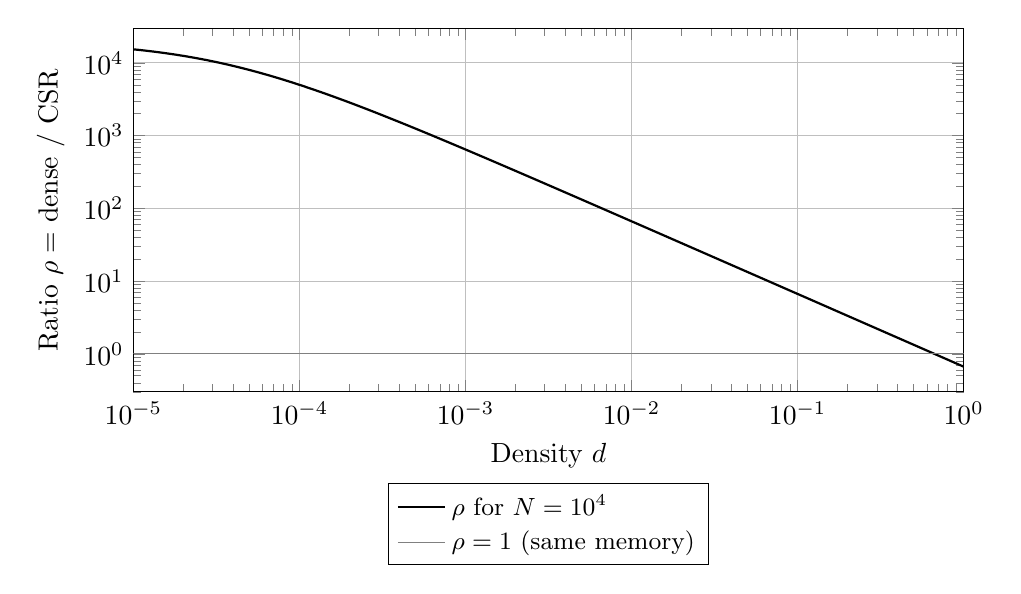
\begin{tikzpicture}
\begin{loglogaxis}[
  width=\textwidth, height=6.2cm,
  xmin=1e-5, xmax=1, ymin=0.3, ymax=3e4,
  xlabel={Density $d$},
  ylabel={Ratio $\rho = $ dense / CSR},
  grid=major, legend cell align=left,
  legend style={at={(0.5,-0.25)}, anchor=north, font=\small}]
\addplot[thick, domain=1e-5:1, samples=80] {8e8/(1.2e9*x + 40004)};
\addlegendentry{$\rho$ for $N = 10^4$}
\addplot[thin, gray, domain=1e-5:1, samples=2] {1};
\addlegendentry{$\rho = 1$ (same memory)}
\end{loglogaxis}
\end{tikzpicture}

\small (b) Memory ratio against density, $N = 10^4$.
\end{minipage}
\caption{Storage of dense and CSR matrices. (a) With a fixed number of
nonzeros per row, dense memory grows as $N^2$ and crosses 16 GB near
$N = 4.5 \cdot 10^4$, while CSR grows linearly. (b) For a fixed size, CSR
saves memory as long as $d < 2/3$; the saving is a factor of about
$2/(3d)$ for small $d$.}
\label{fig:storage}
\end{figure}

%======================================================================
\section{Algorithms}
%======================================================================

\subsection{Dense, row-oriented (dot-product form)}

Natural for row-major storage: each $y_i$ is the dot product of row $i$
with $x$. The inner loop reads $A$ and $x$ contiguously.

\begin{algorithm}[H]
\caption{Dense $y = Ax$, row-major storage}
\label{alg:dense-row}
\begin{algorithmic}[1]
\Require $A[0..MN-1]$ row-major, $x[0..N-1]$
\Ensure $y[0..M-1]$
\For{$i \gets 0$ \textbf{to} $M-1$}
  \State $s \gets 0$
  \For{$j \gets 0$ \textbf{to} $N-1$}
    \State $s \gets s + A[iN + j] \cdot x[j]$
  \EndFor
  \State $y[i] \gets s$
\EndFor
\end{algorithmic}
\end{algorithm}

\subsection{Dense, column-oriented (axpy form)}

Natural for column-major storage: $y$ is built as a linear combination of the
columns of $A$, $y = \sum_j x_j\, a_{:,j}$. Each step is an \emph{axpy}
($y \gets y + \alpha a$).

\begin{algorithm}[H]
\caption{Dense $y = Ax$, column-major storage}
\label{alg:dense-col}
\begin{algorithmic}[1]
\Require $A[0..MN-1]$ column-major, $x[0..N-1]$
\Ensure $y[0..M-1]$
\For{$i \gets 0$ \textbf{to} $M-1$}
  \State $y[i] \gets 0$
\EndFor
\For{$j \gets 0$ \textbf{to} $N-1$}
  \State $\alpha \gets x[j]$
  \For{$i \gets 0$ \textbf{to} $M-1$}
    \State $y[i] \gets y[i] + A[i + jM] \cdot \alpha$
  \EndFor
\EndFor
\end{algorithmic}
\end{algorithm}

\noindent Both forms do the same arithmetic. What matters is that the inner
loop walks through $A$ in the order it is stored; using the wrong loop order
for the storage makes every access to $A$ jump by $N$ (or $M$) elements and
destroys cache efficiency.

\subsection{CSR}

The same dot-product form as \cref{alg:dense-row}, but the inner loop visits
only the $n_i$ nonzeros of row $i$, and reads $x$ through the column index.

\begin{algorithm}[H]
\caption{CSR $y = Ax$}
\label{alg:csr}
\begin{algorithmic}[1]
\Require $\id{row\_ptr}[0..M]$, $\id{col}[0..\nnz-1]$, $\id{val}[0..\nnz-1]$, $x[0..N-1]$
\Ensure $y[0..M-1]$
\For{$i \gets 0$ \textbf{to} $M-1$}
  \State $s \gets 0$
  \For{$k \gets \id{row\_ptr}[i]$ \textbf{to} $\id{row\_ptr}[i+1]-1$}
    \State $s \gets s + \id{val}[k] \cdot x[\id{col}[k]]$ \Comment{indirect access to $x$}
  \EndFor
  \State $y[i] \gets s$
\EndFor
\end{algorithmic}
\end{algorithm}

\noindent An empty row ($\id{row\_ptr}[i] = \id{row\_ptr}[i+1]$) skips the
inner loop and correctly produces $y_i = 0$.

\subsection{Trace on the running example}

\begin{center}
\begin{tabular}{cccl}
\toprule
$i$ & $k$ range & terms & $y_i$ \\
\midrule
0 & 0--1 & $10\cdot x_0 + 2\cdot x_4 = 10 + 10$ & 20 \\
1 & 2 & $3\cdot x_1$ & 6 \\
2 & none ($3$ to $2$) & empty row & 0 \\
3 & 3--4 & $7\cdot x_2 + 1\cdot x_5 = 21 + 6$ & 27 \\
4 & 5 & $4\cdot x_0$ & 4 \\
5 & 6--7 & $5\cdot x_3 + 6\cdot x_5 = 20 + 36$ & 56 \\
\bottomrule
\end{tabular}
\end{center}

\noindent So $y = (20, 6, 0, 27, 4, 56)^{\mathsf T}$. The dense algorithm
performs $2MN = 72$ floating-point operations, 56 of them on zeros; CSR
performs $2\,\nnz = 16$, all useful.

%======================================================================
\section{Cost analysis}
%======================================================================

\subsection{Floating-point operations}

Each stored entry contributes one multiplication and one addition:
\[
  W_{\text{dense}} = 2MN, \qquad W_{\text{CSR}} = 2\,\nnz = 2\,d\,MN .
\]
CSR does a fraction $d$ of the dense work.

\subsection{Memory traffic}

Each entry of $A$ is used exactly once, so $A$ must always be streamed from
main memory (for matrices larger than the cache). The vectors behave
differently:

\begin{itemize}
  \item $y$: written once, $s_v M$ bytes.
  \item $x$, dense: read contiguously and reused by every row; if it stays in
        cache it costs $s_v N$ bytes in total.
  \item $x$, CSR: read through $\id{col}[k]$. In the \emph{best case} (good
        locality, $x$ stays in cache) it costs $s_v N$ bytes; in the
        \emph{worst case} every access misses cache and it costs about
        $s_v\,\nnz$ bytes (even more if each miss loads a whole 64-byte cache
        line for one useful value).
\end{itemize}

\begin{center}
\begin{tabular}{lll}
\toprule
Data & Dense (bytes) & CSR (bytes) \\
\midrule
Matrix values & $8MN$ & $8\,\nnz$ \\
Index arrays & -- & $4\,\nnz + 4(M+1)$ \\
$x$ (best / worst) & $8N$ & $8N$ \ / \ $8\,\nnz$ \\
$y$ & $8M$ & $8M$ \\
\midrule
Total, best case & $8MN + 8M + 8N$ & $12\,\nnz + 12M + 8N + 4$ \\
Total, worst case & -- & $20\,\nnz + 12M + 4$ \\
\bottomrule
\end{tabular}
\end{center}

\subsection{Arithmetic intensity}

The arithmetic intensity $I = W / Q$ (flops per byte moved) decides whether a
computation is limited by the processor or by memory. Keeping only the
dominant terms:
\[
  I_{\text{dense}} \approx \frac{2MN}{8MN} = \frac{1}{4}, \qquad
  I_{\text{CSR}}^{\text{best}} \approx \frac{2\,\nnz}{12\,\nnz} = \frac{1}{6}, \qquad
  I_{\text{CSR}}^{\text{worst}} \approx \frac{2\,\nnz}{20\,\nnz} = \frac{1}{10}.
\]
Every value read from $A$ is used for exactly two flops, and there is no way
to reuse it: unlike matrix--matrix multiplication, $y = Ax$ cannot be
restructured to raise its intensity. CSR has a slightly \emph{lower} intensity
than dense because each value carries a 4-byte index.

%======================================================================
\section{Performance model: the roofline}
%======================================================================

The roofline model bounds the attainable rate by
\[
  P = \min(\pi,\ I\,\beta).
\]
Modern processors have $\pi / \beta$ (the \emph{ridge point}) between about 5
and 20 flop/byte. Since $I \le 1/4$ for both formats, $y = Ax$ is
\emph{memory-bound}: the run time is essentially
\[
  T \approx \frac{Q}{\beta}.
\]

\begin{figure}[H]
\centering
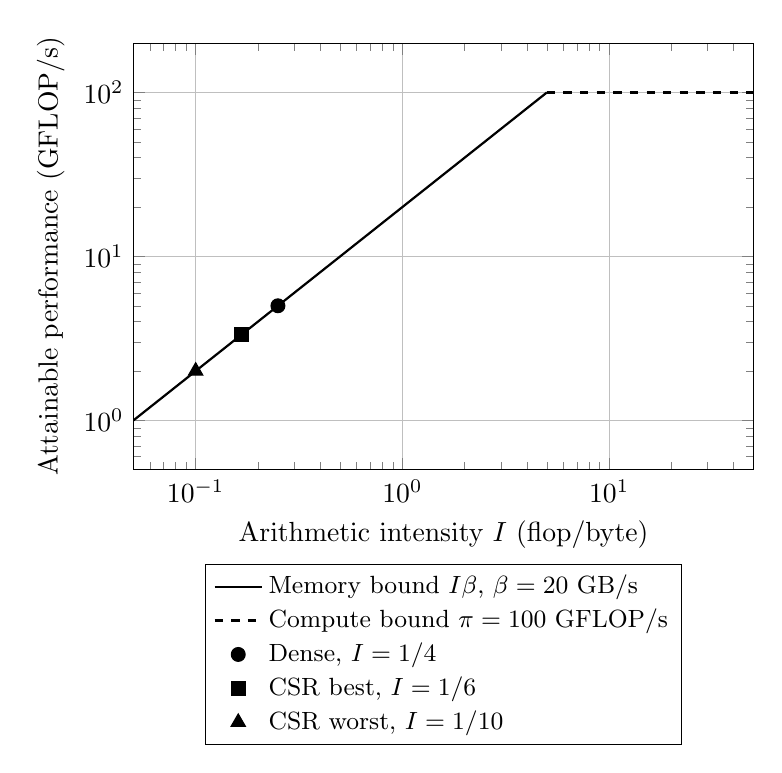
\begin{tikzpicture}
\begin{loglogaxis}[
  width=0.78\textwidth, height=7cm,
  xmin=0.05, xmax=50, ymin=0.5, ymax=200,
  xlabel={Arithmetic intensity $I$ (flop/byte)},
  ylabel={Attainable performance (GFLOP/s)},
  grid=major, legend cell align=left, legend style={at={(0.5,-0.22)}, anchor=north, font=\small}]
\addplot[thick, domain=0.05:5, samples=2] {20*x};
\addlegendentry{Memory bound $I\beta$, $\beta = 20$ GB/s}
\addplot[thick, dashed, domain=5:50, samples=2] {100};
\addlegendentry{Compute bound $\pi = 100$ GFLOP/s}
\addplot[only marks, mark=*, mark size=2.5pt] coordinates {(0.25,5)};
\addlegendentry{Dense, $I = 1/4$}
\addplot[only marks, mark=square*, mark size=2.5pt] coordinates {(0.1667,3.333)};
\addlegendentry{CSR best, $I = 1/6$}
\addplot[only marks, mark=triangle*, mark size=3pt] coordinates {(0.1,2)};
\addlegendentry{CSR worst, $I = 1/10$}
\end{loglogaxis}
\end{tikzpicture}
\caption{Roofline for an illustrative machine ($\beta = 20$ GB/s,
$\pi = 100$ GFLOP/s). Both formats sit far left of the ridge point
($I = 5$): they use at most 5\% of the peak floating-point rate.}
\label{fig:roofline}
\end{figure}

\noindent The \emph{rate} of CSR (flop/s) is a little lower than that of dense,
but CSR does a factor $d$ fewer flops, so its \emph{time} is far smaller.

\subsection{Examples}

All times use $T \approx Q / \beta$ with $\beta = 20$ GB/s and the best-case
CSR traffic.

\begin{center}
\begin{tabular}{lrrrr}
\toprule
Case & \multicolumn{2}{c}{Dense} & \multicolumn{2}{c}{CSR} \\
\cmidrule(lr){2-3}\cmidrule(lr){4-5}
 & traffic & time & traffic & time \\
\midrule
$N = 10^4$, $d = 10^{-2}$ ($\nnz = 10^6$) & 800 MB & 40 ms & 12.2 MB & 0.6 ms \\
$N = 10^6$, $\nnz = 5\cdot 10^6$ & 8 TB & 400 s & 80 MB & 4.0 ms \\
\bottomrule
\end{tabular}
\end{center}

\noindent In the second case the dense matrix does not even fit in the memory
of a workstation; in the first, CSR is about 65 times faster.

%======================================================================
\section{Break-even density}
\label{sec:breakeven}
%======================================================================

Setting the best-case CSR traffic equal to the dense traffic and keeping
dominant terms,
\[
  12\,\nnz \approx 8MN
  \quad\Longrightarrow\quad
  d^{*}_{\text{best}} \approx \frac{2}{3},
  \qquad\text{and with worst-case $x$ traffic,}\qquad
  d^{*}_{\text{worst}} \approx \frac{8}{20} = 0.4 .
\]
Below $d^*$, CSR moves fewer bytes and is faster in this model.

\begin{figure}[H]
\centering
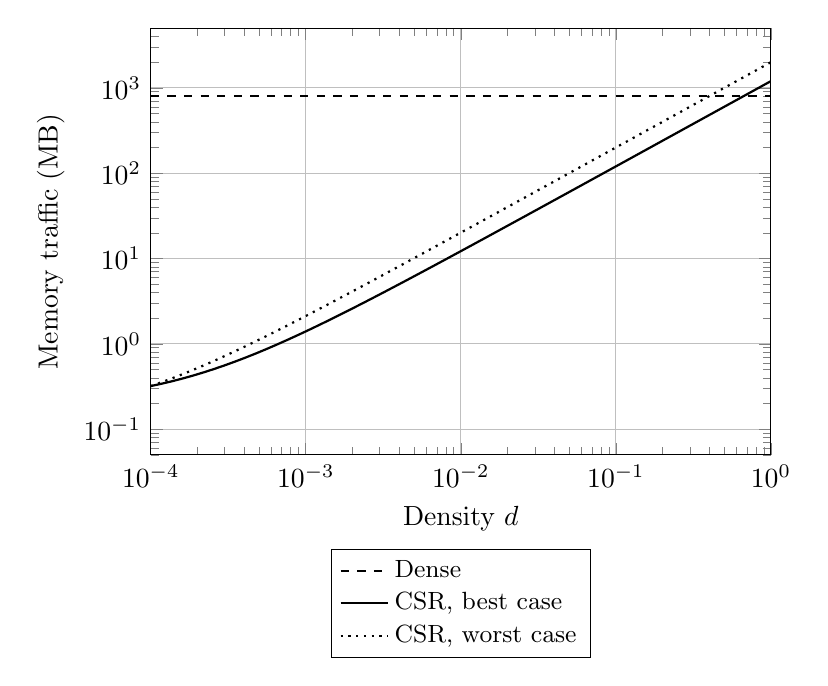
\begin{tikzpicture}
\begin{loglogaxis}[
  width=0.78\textwidth, height=7cm,
  xmin=1e-4, xmax=1, ymin=0.05, ymax=5000,
  xlabel={Density $d$},
  ylabel={Memory traffic (MB)},
  grid=major, legend cell align=left, legend style={at={(0.5,-0.22)}, anchor=north, font=\small}]
\addplot[thick, dashed, domain=1e-4:1, samples=2] {800.16};
\addlegendentry{Dense}
\addplot[thick, domain=1e-4:1, samples=60] {1200*x + 0.2};
\addlegendentry{CSR, best case}
\addplot[thick, dotted, domain=1e-4:1, samples=60] {2000*x + 0.12};
\addlegendentry{CSR, worst case}
\end{loglogaxis}
\end{tikzpicture}
\caption{Memory traffic of one product $y = Ax$ for $M = N = 10^4$. The curves
cross at $d \approx 0.67$ (best case) and $d \approx 0.4$ (worst case).}
\label{fig:breakeven}
\end{figure}

\noindent In practice the crossover is lower than the model predicts, because
the dense inner loop vectorizes perfectly with SIMD instructions and is
prefetched by hardware, while the CSR loop has an indirect access, a short
trip count for short rows, and loop overhead per row. A common rule of thumb
is that CSR pays off below a few percent density; the exact point depends on
the machine and the sparsity pattern and should be measured.

%======================================================================
\section{Memory access patterns}
%======================================================================

\begin{center}
\begin{tabular}{lll}
\toprule
Access & Dense (row-major) & CSR \\
\midrule
$A$ & contiguous stream & contiguous stream (\id{val}, \id{col}) \\
$x$ & contiguous, reused per row & \emph{gather}: $x[\id{col}[k]]$ \\
$y$ & one write per row & one write per row \\
Inner loop length & $N$ (long, uniform) & $n_i$ (short, varies) \\
\bottomrule
\end{tabular}
\end{center}

\noindent The cost of the gather depends on the sparsity pattern:
\begin{itemize}
  \item \textbf{Banded or clustered columns} (e.g.\ discretized PDEs,
        nearby columns in each row): consecutive accesses hit the same cache
        lines, so traffic is close to the best case.
  \item \textbf{Scattered columns} (e.g.\ random graphs, many optimization
        models): accesses miss cache and traffic approaches the worst case.
        Reordering rows and columns (for example with reverse Cuthill--McKee)
        can bring nonzeros closer to the diagonal and improve locality.
  \item \textbf{Very short rows} (1--3 nonzeros): the per-row overhead
        (reading \id{row\_ptr}, starting and ending the loop, writing $y_i$)
        becomes comparable to the useful work.
\end{itemize}

%======================================================================
\section{Parallelization with OpenMP}
%======================================================================

\subsection{Distributing rows}

In both formats the rows are independent: each $y_i$ is written by exactly one
iteration, so the outer loop can be parallelized without synchronization.

\begin{algorithm}[H]
\caption{Parallel CSR $y = Ax$ (one row per iteration)}
\label{alg:csr-par}
\begin{algorithmic}[1]
\For{$i \gets 0$ \textbf{to} $M-1$ \textbf{in parallel}} \Comment{e.g.\ \texttt{omp parallel for}}
  \State $s \gets 0$
  \For{$k \gets \id{row\_ptr}[i]$ \textbf{to} $\id{row\_ptr}[i+1]-1$}
    \State $s \gets s + \id{val}[k] \cdot x[\id{col}[k]]$
  \EndFor
  \State $y[i] \gets s$
\EndFor
\end{algorithmic}
\end{algorithm}

\noindent For dense matrices every row costs the same, so a static schedule
balances the load perfectly. For CSR, rows can have very different lengths
$n_i$. Two common remedies:
\begin{enumerate}
  \item a dynamic or guided schedule, which hands out chunks of rows as
        threads become free (simple, some scheduling overhead);
  \item an \emph{$\nnz$-balanced static partition}: give each thread a
        contiguous block of rows containing about $\nnz/T$ nonzeros
        (\cref{alg:partition}). This keeps the low overhead of a static
        schedule and the memory locality of contiguous blocks.
\end{enumerate}

\begin{algorithm}[H]
\caption{$\nnz$-balanced row partition for $T$ threads}
\label{alg:partition}
\begin{algorithmic}[1]
\Require $\id{row\_ptr}[0..M]$, number of threads $T$
\Ensure $\id{start}[0..T]$: thread $t$ processes rows $\id{start}[t], \dots, \id{start}[t+1]-1$
\State $\id{start}[0] \gets 0$, \quad $\id{start}[T] \gets M$
\For{$t \gets 1$ \textbf{to} $T-1$}
  \State $\tau \gets \lfloor t \cdot \nnz / T \rfloor$
  \State $\id{start}[t] \gets$ smallest $i$ with $\id{row\_ptr}[i] \ge \tau$ \Comment{binary search, $O(\log M)$}
\EndFor
\end{algorithmic}
\end{algorithm}

\noindent A single very long row still cannot be split by this scheme;
merge-based SpMV~\cite{merrill2016} solves that case by splitting the work at
the level of individual nonzeros.

\subsection{Memory placement and threads}

Because the operation is memory-bound, adding threads helps only until the
memory bandwidth is saturated, which often happens before all cores are in
use. On machines with several memory controllers (NUMA), data should be
initialized by the same threads, with the same schedule, that later use it
(\emph{first-touch} placement), and threads should be pinned to cores
(\texttt{OMP\_PROC\_BIND}, \texttt{OMP\_PLACES})~\cite{vanderpas2017}.

\subsection{Vectorization (SIMD)}

The dense inner loop reads contiguous data and vectorizes directly (for
example with \texttt{omp simd reduction(+:s)}). The CSR inner loop needs a
\emph{gather} instruction to load $x[\id{col}[k]]$, which is slower than a
contiguous load, and its short, variable trip count leaves vector lanes
unused. Formats such as SELL-$C$-$\sigma$~\cite{kreutzer2014} rearrange the
nonzeros into fixed-width chunks to improve SIMD and GPU efficiency.

%======================================================================
\section{Numerical considerations}
%======================================================================

Both algorithms compute the same sums, but floating-point addition is not
associative. Dense algorithms add the zero terms (which does not change the
result) and may sum in a different order when vectorized or blocked; parallel
or SIMD versions of either format may also change the order. Results can
therefore differ in the last bits between implementations and between runs
with different numbers of threads. The rounding error bound is the same for
both: $|\hat y_i - y_i| \le \gamma_{n} \sum_j |a_{ij}|\,|x_j|$ with
$\gamma_n = n u / (1 - n u)$, where $u$ is the unit roundoff and $n$ is the
number of terms summed ($N$ for dense, $n_i$ for CSR), so CSR's bound is
never worse.

%======================================================================
\section{Industry-standard implementations}
%======================================================================

\begin{center}
\begin{tabular}{ll}
\toprule
Format & Standard routines \\
\midrule
Dense & BLAS level 2 \texttt{dgemv} (OpenBLAS, BLIS, Intel MKL); \\
      & \texttt{cblas\_dgemv} accepts row- or column-major layout \\
CSR   & Intel MKL Sparse BLAS (\texttt{mkl\_sparse\_d\_mv}); \\
      & NVIDIA cuSPARSE (\texttt{cusparseSpMV}); PETSc (\texttt{MatMult}) \\
\bottomrule
\end{tabular}
\end{center}

\noindent There is no single reference implementation of sparse
matrix--vector multiplication comparable to the reference BLAS for dense
operations; each library uses its own data structures and tuning. A custom
implementation is best validated against one of these libraries, both for
correctness and for speed.

%======================================================================
\section{Summary}
%======================================================================

\begin{center}
\begin{tabular}{lll}
\toprule
 & Dense & CSR \\
\midrule
Storage & $8MN$ & $12\,\nnz + 4(M+1)$ \\
Flops & $2MN$ & $2\,\nnz$ \\
Memory traffic & $\approx 8MN$ & $\approx 12\,\nnz$ to $20\,\nnz$ \\
Arithmetic intensity & $1/4$ & $1/6$ to $1/10$ \\
Bound by & memory bandwidth & memory bandwidth \\
Access to $x$ & contiguous & indirect (gather) \\
Parallel load balance & automatic & needs care if $n_i$ vary \\
SIMD & excellent & limited by gather \\
Faster when & $d$ is large (roughly $> 0.4$ in the model) & $d$ is small \\
\bottomrule
\end{tabular}
\end{center}

\noindent\textbf{Conclusions.}
\begin{enumerate}
  \item $y = Ax$ is memory-bound in both formats; its run time is the number
        of bytes moved divided by the memory bandwidth.
  \item CSR moves about $12\,\nnz$ bytes instead of $8MN$, so for typical
        sparse matrices ($d \ll 1$) it is faster by roughly a factor
        $2/(3d)$, and it makes problems feasible that do not fit in memory
        as dense arrays.
  \item The quality of a CSR implementation depends mostly on the access
        pattern to $x$ and on load balance across threads, not on the
        arithmetic.
\end{enumerate}

%======================================================================
\begin{thebibliography}{9}
%======================================================================

\bibitem{saad2003}
Y.~Saad.
\newblock \emph{Iterative Methods for Sparse Linear Systems}, 2nd ed.
\newblock SIAM, Philadelphia, 2003.

\bibitem{golub2013}
G.~H.~Golub and C.~F.~Van~Loan.
\newblock \emph{Matrix Computations}, 4th ed.
\newblock Johns Hopkins University Press, Baltimore, 2013.

\bibitem{williams2009roofline}
S.~Williams, A.~Waterman, and D.~Patterson.
\newblock Roofline: an insightful visual performance model for multicore
architectures.
\newblock \emph{Communications of the ACM}, 52(4):65--76, 2009.

\bibitem{williams2009spmv}
S.~Williams, L.~Oliker, R.~Vuduc, J.~Shalf, K.~Yelick, and J.~Demmel.
\newblock Optimization of sparse matrix--vector multiplication on emerging
multicore platforms.
\newblock \emph{Parallel Computing}, 35(3):178--194, 2009.

\bibitem{merrill2016}
D.~Merrill and M.~Garland.
\newblock Merge-based parallel sparse matrix--vector multiplication.
\newblock In \emph{Proceedings of SC16}, 2016.

\bibitem{kreutzer2014}
M.~Kreutzer, G.~Hager, G.~Wellein, H.~Fehske, and A.~R.~Bishop.
\newblock A unified sparse matrix data format for efficient general sparse
matrix--vector multiplication on modern processors with wide SIMD units.
\newblock \emph{SIAM Journal on Scientific Computing}, 36(5):C401--C423, 2014.

\bibitem{chapman2007}
B.~Chapman, G.~Jost, and R.~van~der~Pas.
\newblock \emph{Using OpenMP: Portable Shared Memory Parallel Programming}.
\newblock MIT Press, Cambridge, MA, 2007.

\bibitem{vanderpas2017}
R.~van~der~Pas, E.~Stotzer, and C.~Terboven.
\newblock \emph{Using OpenMP -- The Next Step: Affinity, Accelerators,
Tasking, and SIMD}.
\newblock MIT Press, Cambridge, MA, 2017.

\bibitem{boisvert1996}
R.~F.~Boisvert, R.~Pozo, and K.~A.~Remington.
\newblock The Matrix Market exchange formats: initial design.
\newblock NISTIR 5935, National Institute of Standards and Technology, 1996.

\end{thebibliography}

\end{document}
